\chapter{Tecnologías usadas}

Tomando en cuenta la información ya vertida en este documento, a continuación se explicará detalladamente la propuesta de solución.\\
En la figura \ref{fig:4-1-1} se tiene el diagrama general del sistema, se puede apreciar la comunicación entre las diferentes entidades que se usaran, que datos se mandan y reciben y por que canales transitan estos datos. A continuación se describe de manera general como es el proceso de envío y recepción de correos electrónicos ideado para este esquema.\\
\begin{enumerate}
 \item {Envío}
\begin{itemize}
\item El remitente escribe el correo electrónico y le da enviar.\\
\item El correo electrónico pasa por el complemento del cliente de correo.\\
\item El cliente genera a partir del correo una clave que usaremos para cifrar el mensaje.\\
\item Se cifra y se empaqueta el mensaje con el protocolo SMTP.\\
\item Se coloca una bandera en el mensaje.\\
\item La clave se convierte en CAPTCHA y es enviada al servidor de CAPTCHAS.\\
\item Se envía el mensaje de correo electrónico al destinatario.\\
\end{itemize}

\item{Recepción}
\begin{itemize}
\item El receptor abre un correo electrónico cifrado con el presente esquema.\\
\item El cliente lo descarga del servidor por medio del protocolo POP3 o IMAP.\\
\item Se hace una petición al servidor de CAPTCHAS para recuperar los CAPTCHAS del correo.\\
\item El usuario resuelve el CAPTCHA y se recalcula la clave de descifrado.\\
\item Se descifra el mensaje y se le muestra al usuario.\\
\end{itemize}
\end{enumerate}
\begin{figure}[h]
	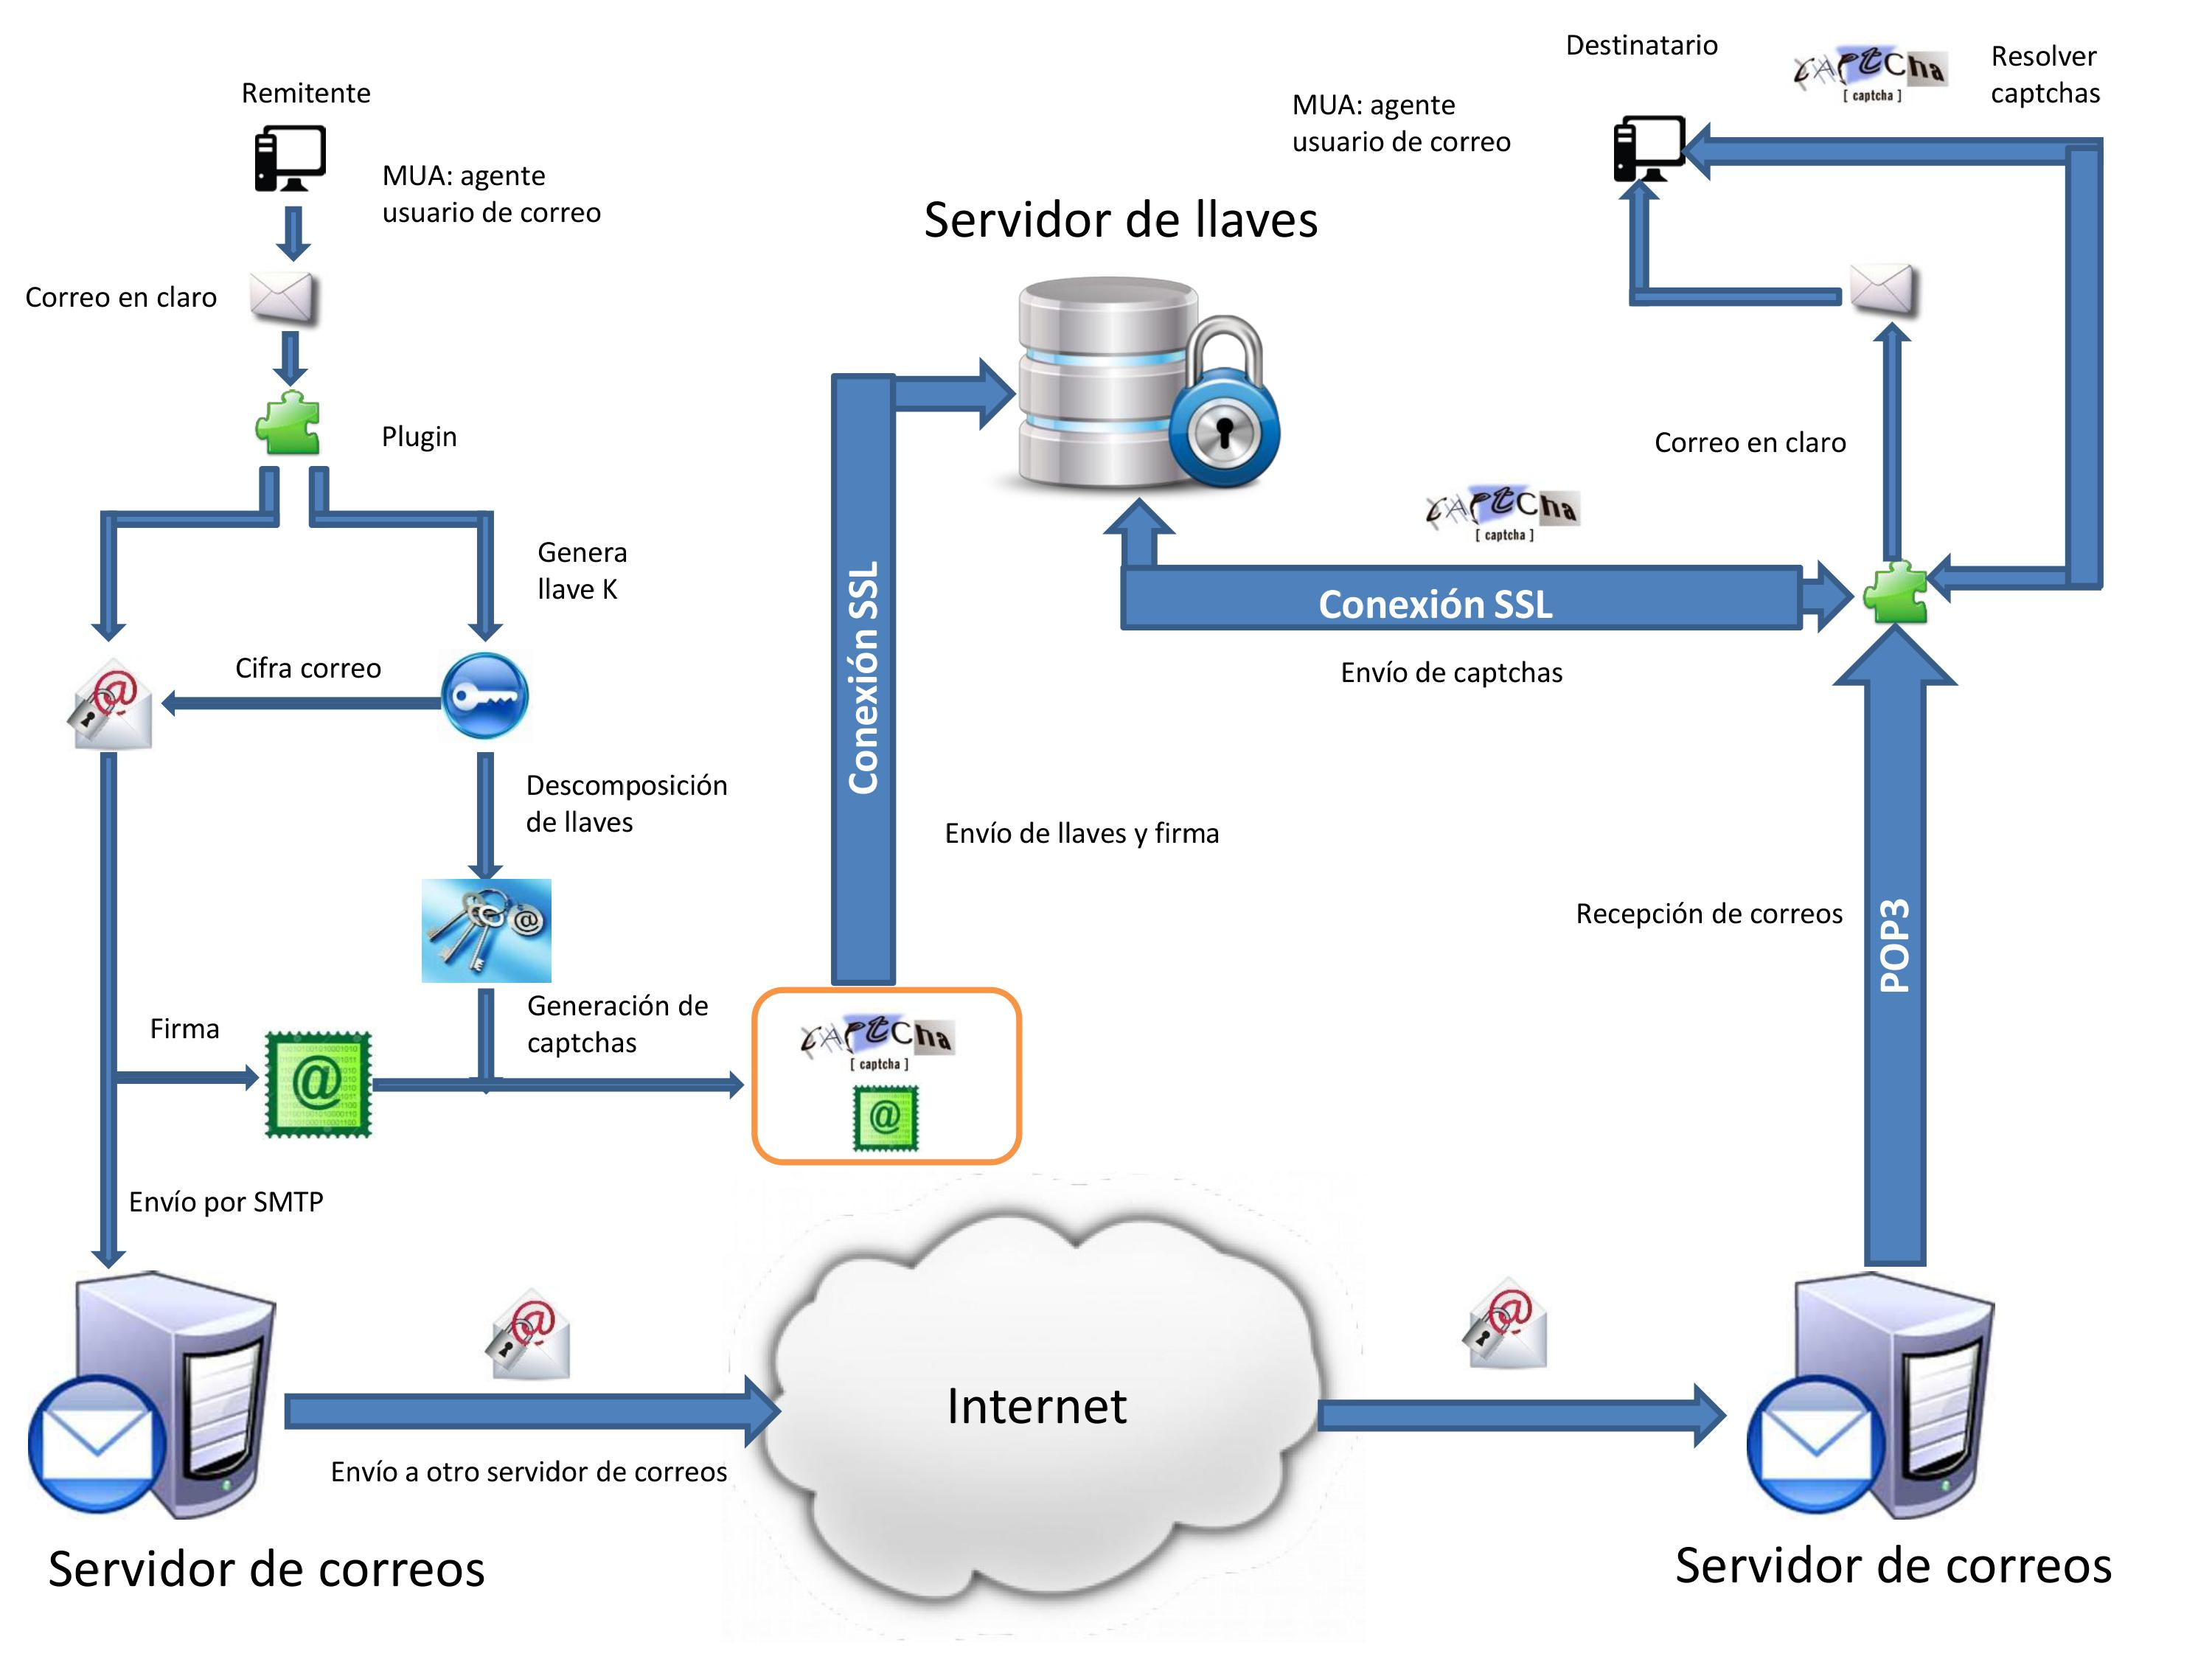
\includegraphics[width=1\linewidth, height=10cm]{./images/0001.jpg}
	\caption{Diagrama General del sistema}
	\label{fig:4-1-1}
\end{figure}
\section{Tecnologías}
Como ya se ha visto en el esquema anterior se necesita hacer uso de las herramientas adecuadas para poder desarrollar este esquema de cifrado. Las herramientas que se analizaron se describen en las siguientes secciones.\\
\subsection{Cliente de correo electrónico}
Un cliente de correo electrónico es necesario para el desarrollo de este proyecto ya que en él se instalará un complemento que cifre el mensaje, envíe los CAPTCHAS y descifre los mensajes de correo electrónico. Para ello buscamos un cliente de correo electrónico que cuente con el soporte de los protocolos POP3, SMTP y IMAP; sus licencias son de código libre; soporte la instalación de APIs externas; y tenga soporte en los sistemas operativos \textbf{\textit{Windows}}, \textbf{\textit{IOS}} y \textbf{\textit{Linux}}. Por lo tanto se investigaron los siguientes clientes de correo electrónico que se encuentra en el mercado: \\
\begin{longtable}[H]{| p{2,5cm} | p{2cm} |p{2cm}|p{1,5cm}|p{2cm}|p{3cm}|p{2cm}|}%\footnotesize
 \hline
 \textbf{Cliente de correo electrónico}&\textbf{Sistema Operativo}&\textbf{Protocolos soportados}&\textbf{Código Libre}&\textbf{Agregar funcionalidad}&\textbf{Extra}&\textbf{Gratuita o de paga}\\
 \hline
 \textbf{eM client}&Windows 7, 8 \& 10 ; IOS&POP3, SMTP, IMAP, EWS, AirSyn&NO&NO&100\% compatible con gmail y sus APIs&Ambos\\
 \hline
 \textbf{Postbox}&Windows, IOS&POP3, SMTP, IMAP&NO&SI por medio de APIs&Sincronización con Dropbox, OneDrive, Facebook y Twitter&Ambos\\
 \hline
 \textbf{Zimbra}&Windows, IOS \& Linux&POP3, SMTP, IMAP&SI&SI por medio de APIs&Una plataforma de nivel empresarial y capas se soportar sincronización con múltiples servicios&Ambos\\
 \hline
 \textbf{Opera Mail}&Windows, IOS \& Linux&POP3, SMTP, IMAP&SI&NO&La plataforma para desarrollar en Opera se actualiza cada semana&Gratuito\\
 \hline
 \textbf{Thunderbird}&Windows, IOS \& Linux&POP3, SMTP, IMAP&SI&SI por medio de APIs&Cliente de correo versátil y fácilmente escalable y una comunicad de desarrollo bastante amplia&Gratuito\\
 \hline
 \textbf{Nylas N1}&Windows, IOS \& Linux&POP3, SMTP, IMAP&SI&Si directamente compilando& &Gratuito
 
    \label{tabla:Descripcion de clientes}
    \\
  \hline

\end{longtable}

\begin{itemize}
 \item El cliente de correo electrónico \textbf{\textit{eM client}} tiene una sincronización a 100\% con las cuentas de \textbf{\textit{Gmail}} y sus APIs, cuenta con una versión gratuita y una versión de paga; puede hacer migración de mensajes de correo electrónico y contactos de diversos clientes de correo electrónico y tiene una compatibilidad con muchos servidores de correo electrónico.\cite{em}\\Su desventaja es que su código es cerrado y permite agregar funcionalidades.
 \item El cliente de correo electrónico \textbf{\textit{Postbox}} esta soportada en los sistemas operativos \textbf{\textit{Windows 7}} o posteriores y \textbf{\textit{IOS}}, esta aplicación es generada por el servidor de correo electrónico \textbf{\textit{Postbox}} por lo tanto cuenta con una sincronización al 100\% con este servidor, también soporta otros servidores de correo como \textbf{\textit{Gmail}} y \textbf{\textit{Outlook}}; este cliente puede sincronizarse con \textbf{\textit{Dropbox}}, \textbf{\textit{Onedrive}} y redes sociales como \textbf{\textit{Facebook}}, \textbf{\textit{Twitter}}, entre otras. Es posible agregar más funcionalidades con la instalación de APIs.\\Una desventaja de esta aplicación es que su código es cerrado, pero gracias a que esta basado en código de \textbf{\textit{Mozilla}} puedes desarrollar APIs para agregarle tus propias funciones. \cite{box}
 \item El cliente de correo electrónico \textbf{\textit{zimbra}} es la aplicación más completa que se analizó, tiene compatibilidad con el servidor \textbf{\textit{zimbra}} pero es capaz de soportar otros servidores de correo electrónico, se encuentra en los 3 sistemas para PC, \textbf{\textit{Windows}}, \textbf{\textit{IOS}} \& \textbf{\textit{Linux}}, da la facilidad de agregarle funcionalidades por medio de la instalación de APIs y gracias a que su código es abierto se pueden programar funciones propias. Este cliente cuenta con la versión gratuita y la versión de paga. Una gran ventaja que tiene es que oferta certificaciones en el desarrollo APIs para este cliente de correo electrónico.\cite{zim}\\La única desventaja que se encontró en este cliente de correo es que la plataforma es demasiado grande y el tiempo que se necesita invertir al estudio del código es demasiado y el tiempo de desarrollo de este proyecto es muy corto.
 \item \textbf{\textit{Opera mail}} es un cliente de correo electrónico que salió al mercado recientemente y se puede instalar en los sistemas operativos \textbf{\textit{Windows}}, \textbf{\textit{IOS}} \& \textbf{\textit{Linux}}, es capaz de comunicarse con diversos servidores de correo electrónico y su código es de libre acceso.\\Su principal desventaja es que las funcionalidades que se quieran agregar no pueden ser adquiridas por medio de la instalación de complementos o APIs.\cite{opera}
 \item Por último tenemos a \textbf{\textit{Thunderbird}} que es un cliente de correo electrónico desarrollado por \textbf{\textit{Mozilla}}, este cliente es de código abierto y la instalación de APIs para agregar funcionalidad es demasiado sencilla; es un cliente de correo que puede ser instalado en los sistemas operativos \textbf{\textit{Windows}}, \textbf{\textit{IOS}} y \textbf{\textit{Linux}}.\cite{thun}
\end{itemize}
Por lo tanto el cliente de correo electrónico que se usará es \textbf{\textit{Thunderbird}}, al ser un cliente de correo electrónico casi tan completo como \textbf{\textit{zimbra}} pero con la facilidad de desarrollar APIs más rápido.\\
\subsection{Lenguajes de programación.}
Uno de los objetivos que se tienen en este proyecto es generar un complemento para un cliente de correo electrónico por lo tanto al escoger a \textbf{\textit{Thunderbird}} como cliente tenemos que programar con el lenguaje que fue desarrollado para tener la mayor compatibilidad.\\Para el desarrollo de este proyecto se utilizará\cite{thun}:
\begin{itemize}
 \item Lenguaje Python
 \item HTML 5
 \item CSS3
\end{itemize}
A pesar de ser una aplicación de escritorio este cliente de correo electrónico está construido con lenguajes web.
\subsection{Tipos de CAPTCHAS}
En el esquema de cifrado es necesario esconder la palabra que genera la clave en un CAPTCHA para ser enviado a otro usuario y descifre el mensaje, pero existen varios tipos de CAPTCHAS que se pueden utilizar\cite{cit}.\\Los CAPTCHAS se pueden clasificar de la siguiente forma:
\begin{itemize}
 \item CAPTCHAS de texto: Este tipo de CAPTCHAS genera una pregunta sencilla donde la respuesta a la pregunta es la respuesta al CAPTCHA.
 \item CAPTCHAS de imágenes: Este tipo de CAPTCHAS nos muestran en una imagen una cadena de caracteres distorsionados, esta cadena de caracteres es la repuesta del CAPCHA transformada en una imagen.
 \item CAPTCHAS de audio: Este tipo de CAPTCHAS se caracterizan por  ser un audio con ruidos de fondo, donde nos dirán la respuesta oculta.
 \item CAPTCHAS de video: Este tipo de CAPTCHAS nos muestran un video de unos cuantos segundos donde una palabra aparece alrededor de la pantalla, esta palabra es la respuesta al CAPTCHA.
 \item CAPTCHAS de acertijos: Este tipo de CPATCHAS es versatil, ya que se trata de pequeños acertijos que resolver donde la respuesta no es una palabra si no una acción o serie de acciones. Los CAPTCHAS de acertijos pueden ser armar un rompecabezas pequeño, seleccionar la imagen que no corresponde, unir figurar geométricas, etc. 
\end{itemize}
Para poder decidir qué tipo de CAPTCHAS se utilizará se consideró los siguientes puntos:
\begin{itemize}
 \item Facilidad de creación.
 \item Peso en bytes del CAPTCHA.
 \item Forma del despliegue.
 \item Tipo de respuesta.
\end{itemize}
Por lo tanto se necesita un tipo de CAPTCHA con poco peso, cuya respuesta sea una cadena de caracteres y su forma de despliegue sea fácil de implementar. \\
Considerando las necesidades anteriores las opciones son CAPTCHAS de imágenes y CAPTCHAS de texto, pero en este proyecto se utilizarán los CAPTCHAS de imágenes porque en ellos seran almacenadas las palabras claves de cifrado de los diferentes mensajes de correo electrónico y estas son cadenas de caracteres que no se les puede generar una pregunta coherente. \\
\subsection{Bases de datos para almacenar los CAPTCHAS.}
Para escoger un gestor de base de datos que controle la información de los usuarios registrados en la aplicación propuesta, la información de los  mensajes que envían entre usuarios y los CAPTCHAS asociados a los mensajes para ser descifrados se consideraron 3 características principales en un gestor base de datos relacional:\\
\begin{itemize}
 \item Rapidez en transferencias de información.
 \item Número de usuarios conectados que soporta.
 \item Facilidad de comunicación entre los lenguajes Python, HTML con los gestores de base de datos.
\end{itemize}
Los 3 gestores que se analizaron fueron SQLite, MySQL y PostGreSQL.\\
SQLite es un gestor de base de datos sumamente ligero que soporta hasta 2 terabytes de información, esta base de datos es compatible con python y lenguajes de programación web. Este gestor por su misma ligereza es posible implementarla en dispositivos móviles, pero no es recomendable cuando múltiples usuarios están haciendo peticiones al mismo tiempo ya que su rendimiento baja\cite{DB}.\\
MySQL es un gestor de base de datos que se caracteriza por su transferencia al hacer consultas de datos almacenados; es uno de los gestores libres más utilizados en aplicaciones web y cuenta con diferentes APIs para hacer la comunicación con los lenguajes Python, PHP, C++, etc. Y soporta peticiones de múltiples usuarios gracias a la implementación de hilos.\\
PostGreSQL es un gestor de base de datos que puede hacer operaciones complejas como subconsultas, transacciones y rollbacks’s. Soporta las peticiones de múltiples usuarios pero en cuanto a la velocidad de transferencia de información, comparado con MySQL, es muy lenta pero lo compensa manteniendo una velocidad casi invariable a pesar de que la base se mantenga con un número grande de registros.\cite{sql}\\
Se eligió el gestor de base de datos MySQL porque el proyecto necesita mayor rapidez en la transferencia de información más que generar filtros muy complejos para la búsqueda de información.\\
\clearpage